\documentclass[sigconf,edbt]{acmart-edbt2020}

\def\BibTeX{{\rm B\kern-.05em{\sc i\kern-.025em b}\kern-.08em
    T\kern-.1667em\lower.7ex\hbox{E}\kern-.125emX}}

\usepackage{booktabs} % For formal tables
\usepackage{subcaption} % 

% Copyright
\setcopyright{rightsretained}

% DOI
\acmDOI{}

% ISBN
\acmISBN{XXX-X-XXXXX-XXX-X}

%Conference
%\acmConference[EDBT 2020]{22nd International Conference on Extending Database Technology (EDBT)}{March 30-April 2, 2020}{Copenhagen, Denmark} 
%\acmYear{2020}

\settopmatter{printacmref=false, printccs=false, printfolios=false}

\pagestyle{empty} % removes running headers

\usepackage{tikz}
\newcommand*\circled[1]{\tikz[baseline=(char.base)]{
            \node[shape=circle,draw,inner sep=2pt] (char) {#1};}}
            

\begin{document}


\title{PML: Stick-Breaking Variational Autoencoders}
%\titlenote{Produces the permission block, and copyright information}
%\subtitle{Extended Abstract}
%\subtitlenote{The full version of the author's guide is available as
 % \texttt{acmart.pdf} document}
  
\author{Laura Mons}
\affiliation{%
  \institution{Technische Universit\"at Berlin}
}
\email{mons@campus.tu-berlin.de}

\author{Stefan Pawlowski}
\affiliation{%
  \institution{Technische Universit\"at Berlin}
}
\email{stefan.pawlowski@infinithings.de}


\author{Tim Korjakow}
\affiliation{%
  \institution{Technische Universit\"at Berlin}
}
\email{tim.korjakow@campus.tu-berlin.de}




% The default list of authors is too long for headers}
% \renewcommand{\shortauthors}{B. Trovato et al.}
\renewcommand{\shortauthors}{}



%
% % The code below should be generated by the tool at
% % http://dl.acm.org/ccs.cfm
% % Please copy and paste the code instead of the example below. 
% %
% \begin{CCSXML}
% <ccs2012>
%  <concept>
%   <concept_id>10010520.10010553.10010562</concept_id>
%   <concept_desc>Computer systems organization~Embedded systems</concept_desc>
%   <concept_significance>500</concept_significance>
%  </concept>
%  <concept>
%   <concept_id>10010520.10010575.10010755</concept_id>
%   <concept_desc>Computer systems organization~Redundancy</concept_desc>
%   <concept_significance>300</concept_significance>
%  </concept>
%  <concept>
%   <concept_id>10010520.10010553.10010554</concept_id>
%   <concept_desc>Computer systems organization~Robotics</concept_desc>
%   <concept_significance>100</concept_significance>
%  </concept>
%  <concept>
%   <concept_id>10003033.10003083.10003095</concept_id>
%   <concept_desc>Networks~Network reliability</concept_desc>
%   <concept_significance>100</concept_significance>
%  </concept>
% </ccs2012>  
% \end{CCSXML}
% 
% \ccsdesc[500]{Computer systems organization~Embedded systems}
% \ccsdesc[300]{Computer systems organization~Redundancy}
% \ccsdesc{Computer systems organization~Robotics}
% \ccsdesc[100]{Networks~Network reliability}


% \keywords{ACM proceedings, \LaTeX, text tagging}

%% A "teaser" image appears between the author and affiliation
%% information and the body of the document, and typically spans the
%% page.
%\begin{teaserfigure}
%  \includegraphics[width=\textwidth]{sampleteaser}
%  \caption{Seattle Mariners at Spring Training, 2010.}
%  \label{fig:teaser}
%\end{teaserfigure}
%!TEX root = paper.tex

\begin{abstract}
Current cloud-based data management systems are not designed for the needs of the upcoming Internet of Things (IoT) applications. In particular, they do not consider heterogeneous setups regarding network topologies and compute nodes. In this demonstration, we showcase one representative use case for the IoT, i.e., a public transport system of a city, and describe its unique challenges. We point out why state-of-the-art data management systems do not qualify for this task and demonstrate NebulaStream (NES) as a system designed for IoT applications. NES unifies data processing techniques from cloud and fog-based systems. By considering the physical network topology and available compute resources, NES minimizes network traffic, and avoids resource over-utilization. Our application on top of NES allows visitors to deploy ad-hoc queries and explore different processing modes. Overall, we show that NES enables future IoT applications that are not realizable with current state-of-the-art systems.
\end{abstract}

\maketitle


%!TEX root = paper.tex
\section{Introduction}
\label{sec:intro}

\cite{nalisnick2016stickbreaking}

\cite{dasgupta_deep_2018}
% 



%!TEX root = paper.tex
\begin{figure}[h]
  \centering
  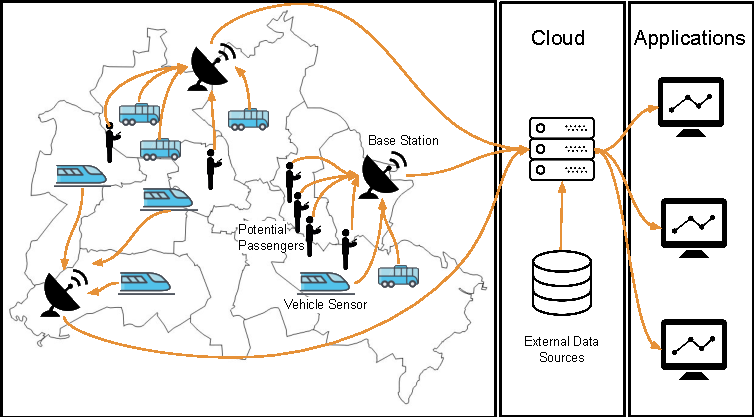
\includegraphics[width=\linewidth]{figs/iot_scenario}
  \caption{Common IoT Infrastructure.}
  \label{fig:iot-app-scenario}
\end{figure}
\section{Data Management in the IoT}
\label{iot}
% 
% In this section, we discuss present our demonstrated IoT use case and point out why state of the art cloud-based SPEs fall short to address those.
% 
% \subsection{Public Transport as an IoT Scenario}
Today's data management application scenarios in the IoT cover a broad range, e.g., failure prediction and anomaly detection in factories, training models for self-driving cars, or tracking of supply chains. 
In the following, we present a representative IoT scenario, and describe the challenges associated with query processing.
In general, IoT scenarios comprise of moving or static sensors connected to the cloud through multiple intermediate nodes.

\subsection{IoT Application Scenarios}
In \Cref{fig:iot-app-scenario}, we show a public transport system as a representative IoT application. 
In this system, vehicles and potential public transport passengers with attached sensors move around the city.
Sensors transmit their data in regular time intervals to geographically distributed base stations, which forward sensor data to the cloud. 
The base stations, as well as the vehicles, represent intermediate nodes in the IoT infrastructure.
On the cloud, sensor streams are subject to enrichment from external sources, e.g., weather or air pollution data.
The resulting data streams are then fed into applications, to answer ad-hoc user queries, to visualize data in GUIs, or to perform advanced analytics.
If a city would implement such an IoT infrastructure, it would enable smart city optimizations such as:
\begin{itemize} 
	\item Reduce air pollution by traffic light control mechanisms.
	\item Ad-hoc route planning to cope with sudden traffic jams.
	\item Automate schedule updates for the public transport based on crowdedness.
\end{itemize}
\textcolor{red}{Laura: Was machen wir an dieser Stelle mit Prof. Markls feedback?}
% 
% \subsection{Fast Decision Taking}
% Datasets of collected sensor data can either be processed in a static or in a dynamic way. 
% In IoT scenarios, it does not always make sense to store all sensor data and perform analytics on outdated static datasets. 
% In contrast, it is of great value to be able to analyze data in real time, and to react to detected patterns, either automatically or with human intervention. For example, when detecting areas with high demand or vehicle failures, it is necessary for an employee to schedule new vehicles.
% \textcolor{red}{(@TODO,der Absatz macht für mich keine Sinn, würde ihn rausnehmen, was willst du denn hier sagen?)}

\subsection{IoT Infrastructure Challenges}
In the following, we discuss challenges related to data management in the IoT. 
Zeuch et al. \cite{nes} point out, that cloud-based SPEs rely on assumptions that IoT infrastractures violate.
First, both paradigms introduce different network topologies.
In particular, processing nodes in cloud-based SPEs are densely connected, i.e., each node can communicate with all other nodes.
In contrast, IoT infrastructures follow a structure similar to p2p networks, where the physical network topology predefines the paths from data sources (sensors) to data sinks (cloud). 
Therefore, every node accesses only a subset of data routed through it. 
For example, a base station located in the west of a city is not able to directly access sensor streams that sensors generate in the east of said city. 
In today's IoT infrastructures, there are orders of magnitude more sensors than nodes. Hence, this physical setup forms a tree-like graph where data flows from sensors among the intermediate nodes to a sink in the cloud.
Finally, when considering multiple layers of intermediate nodes, there might be multiple paths from the source to the cloud. 
Second, both paradigms expect differently sized input streams.
In the fog infrastructure, millions of sensors constantly produce small data streams that capture physical phenomena, such as earthquakes. 
In contrast, cloud-based SPEs are built around the assumptions that few, large data streams, or utilized data brokers (e.g., Kafka) produce them as an input. \textcolor{red}{Laura: Produce what as an input? Bleibt leider auch bei mehrmaligem Lesen unklar.}
% Intermediate nodes are used to transfer data from sensors to the cloud.
% Thus, intermediate nodes are part of the physical environment, e.g., mobile phones, base stations, routers, system-on-a-chip devices, or even regular servers.
%In contrast to robust cloud network infrastructures, network connections in the IoT range from high-speed Ethernet connections to unstable LoWPAN networks and Bluetooth connections. 
%Additionally, nodes constantly change their geospatial location and might cause transient failures, e.g., a bus driving through a tunnel.
% 
%\textbf{Optimizing Across Queries and Operators.}
%IoT applications support two major types of queries, long-running and ad-hoc. 
%Modern SPEs scale-out computation for a large number of queries. However, they only possess minor capabilities to optimize across queries, e.g., when sharing a set of common predicates. 
%Furthermore, some queries have to handle a state (intermediate results) of considerable size, e.g., for window aggregations. 
%However, intermediate IoT nodes provide commonly only restricted storage capabilities.
%This problem is magnified when scaling the number of queries. 
%Therefore, it is necessary for IoT data management platforms to employ data sharing techniques both among queries and operators, techniques proposed by AStream \cite{astream} and Scotty \cite{scotty}.
%\textcolor{red}{(@TODO,mir ist nich ganz klar, sind das denn jetzt die Punkte die du in deiner Demo addressieren willst?)}

%!TEX root = paper.tex
\section{NebulaStream Platform Overview}
\label{nes}
In this demonstration, we focus on specific aspects of NES and provide a brief overview.
For a detailed description of NES, we refer the reader to our previous work~\cite{nes}.  
First, we outline the limitation of state-of-the-art cloud-based SPEs that prevent them from exploiting upcoming IoT infrastructures \Cref{adapting}.
After that, we describe NES and its architecture in \Cref{nes_arch}.
% 
\subsection{Limitation of State-of-the-art SPEs}
\label{adapting}
In the following, we discuss two important features that limit cloud-based SPEs to support future IoT scenarios.

\textbf{Exploitation of Intermediate Nodes:}
Intermediate nodes route sensor-generated data to the cloud.
In an IoT infrastructure, devices are heterogeneous. They range from low-budget processing devices, such as mobile phones and Raspberry PIs, to standard desktop computers and high-end processing nodes with GPUs. 
Current SPEs are unable to exploit all intermediate nodes, because applications must wait until generated data reaches the cloud. 
For example, consider a simple aggregation task, such as counting the number of potential passengers per geographical area. To execute this task, cloud-based systems would have to wait until intermediate nodes propagate the data to the cloud. However, in the described IoT infrastructure, intermediate nodes can execute this task before the data reaches the cloud.

\textbf{On-demand Data Acquisition:}
If the set of running queries does not require all incoming sensor data streams, it would be possible to avoid these sensor reads by employing acquisitional data processing~\cite{tinydb}. 
Additionally, by adapting the sampling frequency of each sensor based on the query requirements, we can reduce network traffic between sensors, and the cloud further.
For example, a vehicle could potentially acquire, and send its data only if it is located in a certain area.


%\subsection{Design Principles}
%\label{nes_chars}
%\textcolor{red}{(@TODO,remove this)}
%NES overcomes the previously introduced limitations of cloud-based SPEs by adhering to the following design principles: 
%\begin{itemize}
%  \item{NES reuses intermediate results both between and within queries, by operator and query-leve optimizations.}
%  \item{NES handles new queries and topology updates incrementally, instead of restarting deployment.}
%  \item{NES generates hardware-tailored code for heterogeneous processing nodes.}
%  \item{NES handles resource availability transparently by providing configurable SLAs.}
%  \item{NES exposes user-friendly interfaces, letting the user focus on business logic rather than system internals.}
%  \item{Every NES node receives the necessary means to react autonomously in case of failures.}
%\end{itemize}

\subsection{Architecture} 
\label{nes_arch}
In the following, we describe NES's architecture. 
We illustrate the architecture in \Cref{nes_architecture}, and focus only on the components that are related to our application scenario. 
Note that NES provides additional components, however, we omit their descriptions because they are out of the scope of this demonstration. 
We refer the reader to our recent work~\cite{nes} for more details.

\textbf{Optimization Process:} 
External Services, e.g., the visualization application from our scenario, submit queries to NES. NES provides APIs to describe common data processing operations, similarly to state-of-the-art SPEs but with fog-specific extensions. 
The \textit{Query Manager} manages and coordinates incoming queries. 
Query execution in NES proceeds as follows. 
First, NES translates the user queries to logical query plans. 
After that, the plan is handed over to NES's Optimizer. 
The \textit{NES Optimizer} consults the \textit{NES Topology Manager}, which monitors the infrastructure changes, and performance statistics. 
The NES Optimizer then composes the execution plan, which it then deploys to its nodes through the \textit{NES Deployment Manager}.
In case of new queries, or topology updates, the NES Deployment Manager applies required changes in an incremental fashion.

\textbf{Deployment and Execution:}
NES's execution plan maps segmented sub-plans to participating, processing intermediate, or cloud nodes. 
Each segment contains processing instructions (tasks), as well as input, and output information. The NES Deployment Manager is responsible for transmitting the sub-plans to each node. After receiving a sub-plan, a node sets up the necessary connections with other nodes, and starts the execution. 
Each node has its own task scheduler, which uses a thread pool, and assigns tasks alongside I/O operations to its resources. 

\textbf{Monitoring:}
During runtime, the NES Topology Manager monitors the execution, and reacts to changes incrementally, e.g., by transitioning smoothly between execution plans. 
To this end, the NES Topology Manager collects hardware statistics such as CPU, or main memory usage, and application-specific statistics like selectivity, or data distributions.
In NES, nodes are designed to handle a wide range of scenarios autonomously. 
For example, in case of transient network failures, a node is able to change buffer execution strategies, or buffer processed data. 
Once the failed network connections are restored, the changes are propagated to the NES Topology Manager.
% 
\begin{figure}[h]
  \centering
  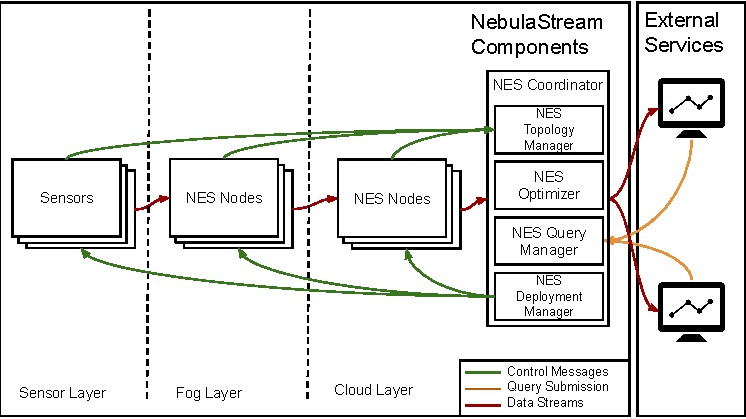
\includegraphics[width=\linewidth]{figs/nes_architecture}
  \caption{Simplified NES architecture overview.}
  \label{nes_architecture}
\end{figure}

Overall, its characteristics allow NES to overcome the limitations of cloud-based SPEs. NES paves the way for a scalable data management back-end for applications in the IoT domain.

%!TEX root = paper.tex
\section{Demonstration}
\label{demo}
We demonstrate NES through an application for public transport. In the following, we describe our user-interface (\Cref{subsec:user_interface}), the setup (\Cref{subsec:setup}), and the application (\Cref{section:application}).

\subsection{User Interface}
\label{subsec:user_interface}
Visitors interact with our application through a GUI, as shown in \Cref{fig:screenshot}. Our GUI consists of an interactive map, which includes moving objects that are either potential passengers, or public transport vehicles (trains, buses, etc.). Our application aims at detecting crowded areas that are covered insufficiently by public transport services, and thus should be re-scheduled by the public transport agency. \textcolor{red}{Laura: What should be re-scheduled. Sentence is a little bit confusing and unclear.}
To this end, the application clusters potential passengers according to their geolocation. When public transport vehicles underserve a cluster of potential passengers, our application notifies the visitor by highlighting the respective map markers. 

Besides its notification mechanism, our GUI allows filtering objects by moving the visible map area, and by selecting vehicle types. The visitor may configure the filters, and the clustering algorithm by changing parameters~\Cref{fig:screenshot}~\circled{1}, such as object distance, or cluster size. 
Furthermore, our GUI also includes performance metrics, such as ad-hoc application statistics~\circled{3} and resource utilization~\circled{4}. 
A main feature of our GUI is choosing between processing modes~\circled{2}. The modes represent the solution space for IoT applications. We aim at showcasing the strengths, and weaknesses of each solution in a hands-on experience.
\begin{figure*}[t!]
  \centering
  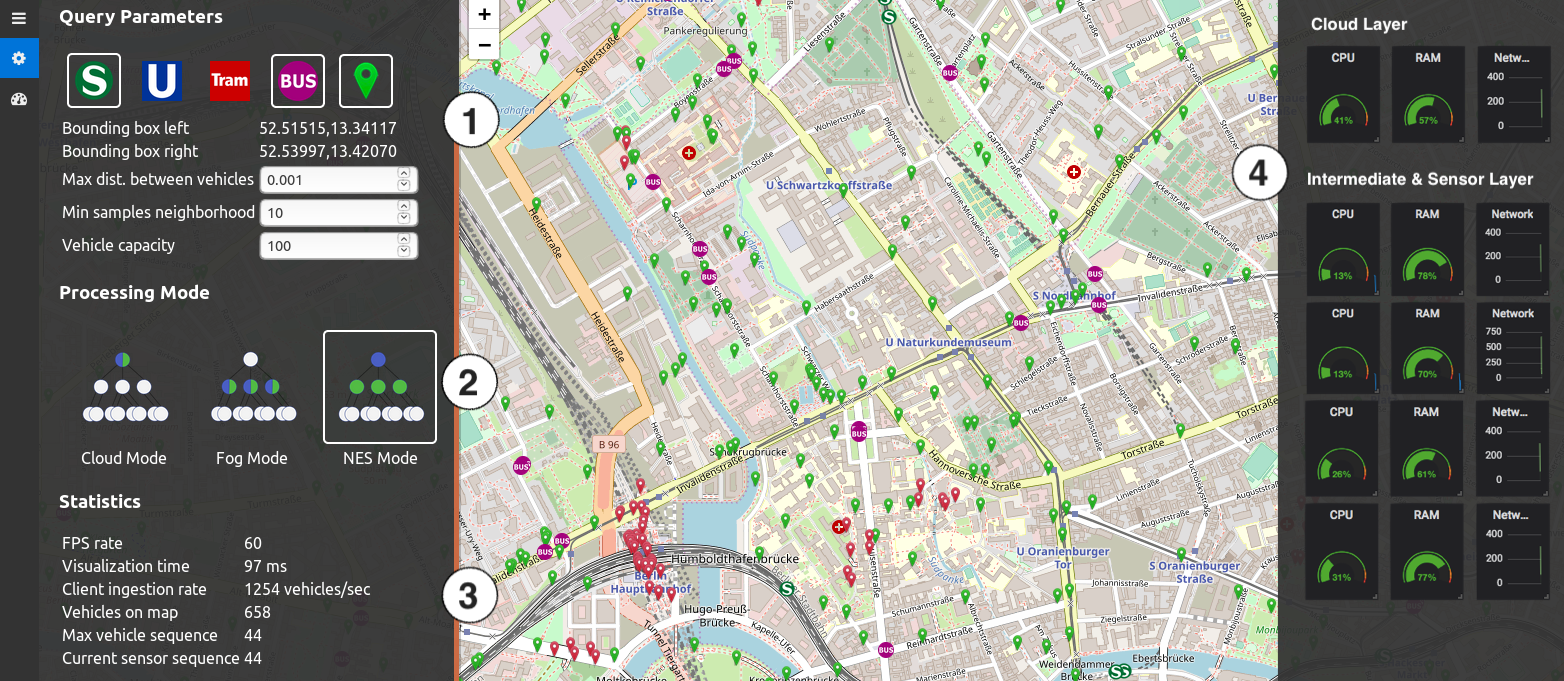
\includegraphics[width=\textwidth]{figs/MapWithClusters_Metrics.png}
  \caption{Demo GUI with potential passengers, buses, and trains. The application clusters potential passengers (green) by area density, and marks clusters red for insufficiently covered areas. The visitor may configure the query parameters (1), the processing modes (2), and observe query information (3) and runtime statistics about resource utilization (4).}
  \label{fig:screenshot}
\end{figure*}


%with the help of DBSCAN \cite{Ester:1996:DAD:3001460.3001507}. DBSCAN clusters the input data based on their closeness. It also provides two parameters to change how DBSCAN defines which objects are close to one another. The first parameter represents the maximal possible distance between two samples, while the second accounts for the minimum number of samples in the neighborhood of a core point. A visitor may change both to explore various cluster scenarios. \\ 

\subsection{Demo Setup}
\label{subsec:setup}

In the following, we describe the setup of our demonstration.

\textbf{Hardware:} For our demonstration scenario, we assume a topology where each public transport vehicle carries a sensor, which transmits its geolocation to a base station, at regular time intervals. Potential passengers also send their geolocation to the base stations, e.g., with a mobile application that uses the sensor attached to a mobile phone. 
For demonstration purposes, we use Raspberry Pis as base stations (fog nodes), and a Laptop as a cloud node. The nodes are interconnected through a router.

\textbf{Software:} Our application consists of a user frontend, and a webserver which uses NES as its execution engine for data processing. The webserver acts as an intermediator between multiple user frontends, and NES. It coordinates query transmission to NES, and forwards query results to our frontends.
Our application backend is written in Python, and uses the Flask microframework. The frontend is implemented in Javascript, and utilizes websockets to communicate with the webserver. We employ the Leaflet framework to implement our interactive map.

\textbf{Dataset:} We simulated two sensor types to compose the dataset for our demonstration.
First, we simulate vehicle sensor data directly at the base stations using real-world \textit{General Transit Feed Specification} datasets~\cite{gtfs}.
Second, we simulate potential passengers using the \textit{Simulation of Urban Mobility} (SUMO) generator~\cite{sumo}. 
We partition both datasets by geolocation, to resemble geographically distributed base stations.
The sensor records contain the measured time, and information about each measurement, such as sensor geolocation, and vehicle type. \textcolor{red}{Laura: Each measurement passt hier irgendwie nicht so gut. Vielleicht lieber: ... and additional information, such as sensor geolocation ...}

\subsection{Application}
\label{section:application}
In our demonstration, we highlight two aspects of a data management system for the IoT.
First, we showcase the deployment process that takes submitted ad-hoc queries from a user interface as input, and deploys operators on the processing nodes to answer this query.
Secondly, we demonstrate the query execution process in NES, by deploying different execution plans, and revealing their implications on resource utilization.
% We use the remainder of this section to further describe those aspects.

\subsubsection{Query Deployment}
%The use case of this application is to detect underserved areas based on crowdedness. 
%We show NES's potential as we deploy the visitor's inputs from the application's interface to NES queries by reducing data as early as possible in the IoT Network. Especially in visualization scenarios reducing data is key for performance issues as well as responsiveness. To fulfill this purpose, NES provides the possibility to filter data needed for visualization purposes as early as in the Fog Layer. Therefore, it not only reduces the data send to the visualization application but the overall network traffic.
%Once a user interacts with the GUI, NES receives a query including parameters for the following three operations:
% 
The main goal of our application is to detect underserved areas based on crowdedness. 
In this application, NES allows us to reduce data as early as possible in the IoT infrastructure. 
Especially in visualization scenarios, data reduction is a key performance factor, and naturally occurs because users are seldomly interested in the entire data set.
To this end, NES provides the option to filter data needed for visualization purposes already in the intermediate (fog) layer. 
The resulting data reduction is two-fold. 
First, NES uses on-demand data acquisition techniques to only gather sensor data that is currently required to answer the query.
Seconds, NES uses intermediate nodes to evict unnecessary data close to the sensors.
Both data reductions minimize the overall network traffic inside the IoT infrastructure, as well as data that has to be sent to applications, in our case the web server.

In our demonstration, the application sends a new query to NES, every time a visitor interacts with the map and its options. A visitor interaction on the map creates a new query that consists of the following parametrized operations:
\begin{itemize}
  \item \textbf{Map Bounding Box:} This parameter filters \textcolor{red}{Laura: These parameters filter ... (es sind ja mehrere Parameter)} the vehicles, and potential passengers located within a bounding box. The bounding box depends on the map area currently viewed by the visitor.
  \item \textbf{Vehicles and Passengers:} This parameter \textcolor{red}{Laura: Same as above} filters passengers, and selected vehicle types, e.g., bus, train, or subway.
  \item \textbf{Clustering:} This parameter adjusts \textcolor{red}{Laura: Same as above} the specifications for our clustering algorithm (DBSCAN~\cite{dbscan}), such as object distance. The algorithm clusters the previously filtered sensor records, and yields the underserved areas. 
\end{itemize}

%Therefore, NES retrieves information to reduce the data load from the interface through queries. 
%Every time a visitor interacts with the map and its options, the application sends a new query to NES. Those queries include parameters to define the currently selected map part, and visitor's selection of vehicle types. 
%In each case, NES limits the processed and send data load to adhere to the requested parameters. 
% We implement our crowdedness algorithm and filtering operations on NES, which reduces the data amounts transferred to the user interface.
% The application itself includes a webserver, that is accessible by multiple clients, i.e. web browsers.
% Mapping the user interface with queries
%NES takes this query and applies it onto the given topology.
% NES takes care of data management operations, while in the application we focus only on implementing the business logic.%, in our case filtering vehicles and highlighting crowded clusters.
%In our application, we use NES as a data management backend, and forward only necessary data to our application.
% 
\subsubsection{Query Execution}
% 
In \Cref{nes}, we introduced the NES Optimizer, which produces, and evaluates potential execution plans.
Each execution plan contains a mapping of NES operators to nodes in the IoT infrastructure.
The optimizer would come up with three execution plans that resemble cloud-based, fog-based, and unified approaches, which we refer to as processing modes.
Note that in our demonstration, we use NES to reproduce all processing modes.
% 
In ~\Cref{fig:screenshot}~\circled{2}, we present these modes, marking filter operations with green color, and clustering operations with blue color.
In our demonstration, visitors can choose between the following three processing modes:
%\nointent 
% \begin{figure*}[t!]
%   \centering
%    \begin{subfigure}[t]{0.339\textwidth}
%         \centering
%         \includegraphics[width=\textwidth]{figs/Cloud_mode_ut.png}
%         \caption{Cloud Mode.}
%     \end{subfigure}%
%     ~ 
%     \begin{subfigure}[t]{0.28\textwidth}
%         \centering
%         \includegraphics[width=\textwidth]{figs/Fog_mode_ut.png}
%         \caption{Fog Mode.}
%     \end{subfigure}%
%     ~ 
%     \begin{subfigure}[t]{0.277\textwidth}
%         \centering
%         \includegraphics[width=\textwidth]{figs/NES_mode.png}
%         \caption{NES Mode.}
%     \end{subfigure}%
%   \caption{Processing modes supported by NES. Green nodes process the filter operation. Blue nodes process the clustering operation. Red nodes represent high CPU and RAM utilization. Red connections mark high incoming network traffic.}
%   \label{fig:execution-plans}
% \end{figure*}

\begin{itemize}
  \item \textbf{Cloud Mode:} The cloud mode represents the processing of current cloud-based SPEs. NES places all operators on the cloud nodes. Performance metrics will reveal that the main workload gathers in the cloud layer while the processing resources of the intermediate fog nodes remain unused.
  \item \textbf{Fog Mode:} NES places all operators on the intermediate layer. The visitor will observe that filtering on the fog reduces network traffic. However, CPU, and RAM usage on the fog nodes increases significantly.
  \item \textbf{NES Mode:} NES places the filter operators on the fog nodes, and the clustering operator on the cloud nodes. The visitor will observe that network traffic, CPU, and RAM utilization remain at a moderate level due to evenly distributed workloads alongside the early filters.
\end{itemize}

In sum, in this demonstration, we highlight the shortcomings of state-of-the-art systems for IoT applications, and the benefits of using NES as a data management platform for IoT scenarios. \textcolor{red}{Laura: Der Satz passt meines Erachtens nach eher in die Conclusion als hier hin, da wir in dieser Sektion nicht auf die shortcomings bzw. benefits von NES eingehen.}
%\textbf{IoT Monitoring.}
%A visitor can monitor the incoming network traffic, RAM and CPU utilization per node on the right in Figure~\ref{fig:screenshot}. %Incoming tuples, 
%The visitor can see: 
% - RAM utilization
% - CPU utilization
% - Tuples incoming
% - Data Ingestion
% of the intermediate layer and the cloud layer.

%\nointent 
%\textbf{Logical Plan}
%- Multiple users/queries are supported.
%- Filtering by Window size. 
%- Filtering by Trasport type.
%- Clustering

%\noindent \textbf{Interactions.} The application can be configured to operate in different modi, in order to allow the visitor to observe performance metrics of various deployment strategies, e.g. saved network traffic during filter push-down. Furthermore, everytime the map is moved, we deploy a new query with the new bounding box parameters, and the new stream is seamlessly ingested by our application.

%!TEX root = paper.tex
\section{Conclusion}
\label{conclusion}
In this paper, we highlighted data processing challenges in the IoT domain, and demonstrated NES, a system that tackles those challenges. We showcased NES through a visualization application for a public transport monitoring system. 
Our application translates user actions on its GUI to NES queries. Using different execution plans, the visitor observes the implications on resource utilization of NES's cross-paradigm operator placements. Using NES as our data management backend, we are able to scale applications in large IoT infrastructures.
% and thus enable new types of IoT applications.


% %!TEX root = paper.tex
\begin{acks}
This work was supported by ...
\end{acks}



%%
%% The next two lines define the bibliography style to be used, and
%% the bibliography file.
\bibliographystyle{ACM-Reference-Format}
\bibliography{paper_references}

%%
%% If your work has an appendix, this is the place to put it.
%% Please note that all the content must fit within the page limits, including any appendices.
%\appendix
%
%\section{Research Methods}
% ...

\end{document}
\endinput
